\documentclass[10pt]{exam}
\usepackage[T1]{fontenc}
\usepackage[paper=a4paper,margin=2cm]{geometry}
\usepackage[sfdefault,light]{roboto}

\usepackage[usenames,dvipsnames]{xcolor}
\usepackage{amsmath,amssymb,array,graphicx,enumitem,listings,lstautogobble,multicol,textcomp,titlesec}
\usepackage{mathtools}

\setlength\parindent{0cm}

%Title & Section Formatting
\titleformat{\section}{\normalfont\Large\bfseries}{}{0em}{}[{\titlerule[0.5pt]}]
\titleformat{\subsection}{\normalfont\large\bfseries}{}{0em}{}

%Mathematical Shortcuts
\newcommand{\floor}[1]{\left\lfloor #1 \right\rfloor}
\newcommand{\ceil}[1]{\left\lceil #1 \right\rceil}

%Listings Shortcuts & Settings
\newcommand{\code}[1]{\lstinline{#1}}
\lstset{language=Java,
        autogobble=true,
        basicstyle=\ttfamily,
        commentstyle=\color{black!45},
        keywordstyle=\bfseries,
        showstringspaces=false,
        upquote=true}

%General Shortcuts
\newcommand{\blankpage}{\null\thispagestyle{empty}\addtocounter{page}{-1}\newpage}


\titleformat{\subsubsection}{\normalfont\bfseries}{}{0em}{}

\header{\footnotesize\scshape Case Study \#\CaseStudyNumber: \CaseStudyTitle}{}{}
\cfoot{\footnotesize\scshape \CaseStudyCourse\\Woodstock School---Mussoorie, Uttarakhand---India}


\def\CaseStudyCourse{AP Computer Science A}
\def\CaseStudyNumber{01}
\def\CaseStudyTitle{Raster Graphics}

\begin{document}
	\begin{coverpages}
		\ \\[2cm]
		\begin{center}
			\huge
			\textbf{Case Study: \CaseStudyTitle}

			\Large
			\CaseStudyCourse
		\end{center}

		\vspace{1.5cm}

		\begin{center}
			\includegraphics[scale=0.45]{graphics/logo_black}

			\vspace{2.5cm}

			\Large
			Name: \rule{11.5cm}{0.1pt}
		\end{center}
	\end{coverpages}

	\blankpage

	\thispagestyle{empty}
	\tableofcontents

	\pagebreak

  \section{Background}
    If you've used a computer, chances are you've taken, stored, transmitted, and edited digital image files. For over half a century, computer scientists and other researchers have developed techniques for the processing of these files. Despite this, every file format designed for storing digital image data can be placed in one of two categories: \emph{raster} and \emph{vector} file formats. Although vector formats are interesting, they are not nearly as common, mostly due to being unsuited for handling complex image data from digital cameras and other image capturing devices. As such, this case-study will focus on the handling of raster graphics.

    \subsection{Raster Graphics}
      A \emph{raster graphic} file format is any digital image file format that arranges its information according to a rectangular grid of pixels. Various file formats have been created that allow for varying degrees of image data compression, colour-depth, and the lossless preservation of image data. These types of image files will typically represent image data as a combination of an indexed palette of colours along with data representing which indexed colour should be reproduced for a given pixel. In memory, these images can then be stored as rectangular arrays of data corresponding to the indices within the colour palette and processed for display on a computer monitor or other display device.\\[\baselineskip]
      A special type of raster image, called a \emph{bitmap}, stores only binary image data. That is, a single bit is used to represent each pixel, with only two colours (typically black and white) available for display.
      %Bit-Mapped & Raster Graphics
    \subsection{Indexed Colours \& Colour Palettes}
      Many raster image files store a \emph{colour palette} alongside the image pixel data to enable more colour-depth. These colour palettes setup an indexed listing of colours that can then be referenced within the image data. The following example shows a 4-colour palette, the corresponding image data, and the corresponding image using this scheme.\\[\baselineskip]
      \begin{minipage}[t]{0.2\textwidth}
        \begin{center}
          \textbf{Colour Palette}
          \ \\[12pt]
          \renewcommand\arraystretch{1.25}
          \begin{tabular}{| p{0.1\textwidth} | c |}
            \hline
            0 & \fcolorbox{black}{black}{\parbox{0.005\textwidth}{\ }} \\
            \hline          
            1 & \fcolorbox{black}{red}{\parbox{0.005\textwidth}{\ }} \\
            \hline          
            2 & \fcolorbox{black}{blue}{\parbox{0.005\textwidth}{\ }} \\
            \hline          
            3 & \fcolorbox{black}{green}{\parbox{0.005\textwidth}{\ }}\\
            \hline          
          \end{tabular}
        \end{center}
      \end{minipage}
      \begin{minipage}[t]{0.4\textwidth}
        \begin{center}
          \textbf{Image Data}
          \ \\[9pt]
          \renewcommand\arraystretch{1.475}
          \ttfamily\footnotesize
          \begin{tabular}{| c | c | c | c | c | c | c | c | c | c | }
            \hline
            0 & 0 & 0 & 0 & 0 & 0 & 0 & 0 & 0 & 0 \\
            \hline         
            0 & 1 & 1 & 1 & 1 & 1 & 1 & 1 & 1 & 0 \\
            \hline         
            0 & 1 & 2 & 2 & 2 & 2 & 2 & 2 & 1 & 0 \\
            \hline         
            0 & 1 & 2 & 3 & 2 & 2 & 3 & 2 & 1 & 0 \\
            \hline         
            0 & 1 & 2 & 2 & 2 & 2 & 2 & 2 & 1 & 0 \\
            \hline         
            0 & 1 & 2 & 3 & 2 & 2 & 3 & 2 & 1 & 0 \\
            \hline         
            0 & 1 & 2 & 2 & 3 & 3 & 2 & 2 & 1 & 0 \\
            \hline         
            0 & 1 & 2 & 2 & 2 & 2 & 2 & 2 & 1 & 0 \\
            \hline         
            0 & 1 & 1 & 1 & 1 & 1 & 1 & 1 & 1 & 0 \\
            \hline         
            0 & 0 & 0 & 0 & 0 & 0 & 0 & 0 & 0 & 0 \\         
            \hline         
          \end{tabular}
        \end{center}
      \end{minipage}
      \begin{minipage}[t]{0.4\textwidth}
        \begin{center}
          \textbf{Displayed Image}
          \ \\[9pt]
          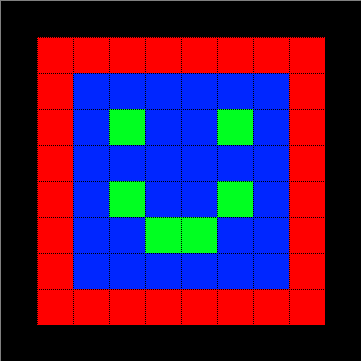
\includegraphics[scale=0.4]{graphics/case_studies/01_RasterImageExample}
        \end{center}
      \end{minipage}
      \ \\[\baselineskip]
      When combined with other data-compression techniques, the use of a colour palette can drastically reduce the size of digital image files containing a limited number of colours ($256$ or less), such as logos, icons, emoticons, etc.
      %Indexed Colours & Colour Palettes
      %%Example of how colour palettes work...
    \subsection{Common Raster Graphic File Formats}
      %Common Raster Graphic formats (TIFF/GIF/PNG/JPG)      
    \subsection{Our File Formats}
      %Simplified file format -- introduction to the case study's file format
      Because traditional image file formats use various forms of compression in order to save hard drive space and decrease transmission times as well as support a number of more advanced features (such as animations and alpha channels), their implementation is beyond the scope of this case study. To that end, the following two file formats have been designed in order to give the student a feel for how to handle binary image data without being bogged down with the individual details that go into advanced image file formats. They may be considered highly simplified versions of some of the more popular raster image file formats.
      \subsubsection{Computer Science Bit-Map File Format}
        %%Computer Science Bit-Map File Format
        %%%'CSBM''w''h''bitmap data'
        In order to distinguish a traditional bit-mapped image from an indexed colour one for this case study, the first four bytes of each bit-map image will contain the ASCII encoded characters: `CSBM' (Decimal: \code{67 83 66 77}). This is known as the file's \emph{signature} and indicates to a program attempting to process the file exactly what type of file is being read.\\[\baselineskip]
        The following two bytes of the file will contain the width and height, respectively.\\
        {\small\textbf{Note:} Because the width and height are each restricted to a single byte of information, the maximum size of an image in this format is $255 \times 255$.}\\[\baselineskip]
        Each of the remaining bits represents the image data as either a $0$ to indicate a black pixel or a $1$ to indicate a white one. Any bits exceeding \emph{width} $\times$ \emph{height} should be ignored.
        \begin{center}
          \renewcommand\arraystretch{1.5}
          \begin{tabular}{| c | c | c | c | c | c | c |}
            \hline
            \code{`C'} & \code{`S'} & \code{`B'} & \code{`M'} & \emph{width} & \emph{height} & \emph{image data}\\
            \hline
          \end{tabular}
        \end{center}

      \subsubsection{Computer Science Indexed Colour File Format}
        %%Computer Science Indexed Colour File Format
        %%%'CSIC''w''h''p''palette''graphic data'
        The signature for the Computer Science Indexed Colour File Format is `CSIC' (Decimal: \code{67 83 73 67}).\\[\baselineskip]
        As with the Computer Science Bit-Map File Format, the following two bytes of the file will contain the width and height, respectively.\\[\baselineskip]
        The next byte will contain the number of elements in the colour palette, $p$. What follows is a group of $3p$ bytes, wherein each set of $3$ bytes contains the values for \emph{red}, \emph{blue}, and \emph{green} making up each color.\\
        {\small\textbf{Note:} For the purposes of this case-study (and most colour indexed file formats), $p$ will be a power of $2$.}\\[\baselineskip]
        Finally, each remaining group of $\lg p$ bits will represent a single pixel of the image. Any bits exceeding \emph{width} $\times$ \emph{height} $\times$ $\lg p$ should be ignored.
        \begin{center}
          \renewcommand\arraystretch{1.5}
          \begin{tabular}{| c | c | c | c | c | c | c | c | c |}
            \hline
            \code{`C'} & \code{`S'} & \code{`I'} & \code{`C'} & \emph{width} & \emph{height} & \emph{palette count} & \emph{palette colours} & \emph{image data}\\
            \hline
          \end{tabular}
        \end{center}
  \pagebreak

  \section{Section \#1} %Handling binary files...
    \subsection{Activity \#1}
      \subsubsection{Introduction}
        %How to read and write binary files.
        %The Java 'byte' primitive.
        %How to read individual bits from a byte.
      \subsubsection{Exercises}
        %Opening the file and reading context information from it.
        %Read and write from a simple bitmap file into a two-dimensional array of bits.
      \subsubsection{Questions}

    \subsection{Activity \#2}
      \subsubsection{Introduction}
        %Dealing with Color objects.
      \subsubsection{Exercises}
        %Read and write binary data from a colour indexed file into a two-dimensional array of Color objects.
      \subsubsection{Questions}

  \pagebreak

  \section{Section \#2} %Defining new colour palettes...
    \subsection{Activity \#3}
      \subsubsection{Introduction}
        %The ColorPreset class.
      \subsubsection{Exercises}    
        %Reading & writing from a ColorPresets file => Activating the "Save Color Palette" button.
        %Modifying the Color[][] array when new presets are selected.
      \subsubsection{Questions}

    \subsection{Activity \#4}
      \subsubsection{Introduction}
        %Different sizes for colour palettes (PNG/GIF options)
      \subsubsection{Exercises}
        %Allowing for larger colour palettes => Dynamically setting up the colour palettes for display.
      \subsubsection{Questions}


  \pagebreak
  
  \section{Section \#3}
    \subsection{Activity \#5} %Simple Transformations
      \subsubsection{Introduction}
        %
      \subsubsection{Exercises}
        %
      \subsubsection{Questions}
        %

    \subsection{Activity \#6} %Colour Transformations
      \subsubsection{Introduction}
        %
      \subsubsection{Exercises}
        %
      \subsubsection{Questions}
        %

  \pagebreak

  \section{Final Analysis}

  \pagebreak

  \section{Template Classes}
\end{document}